\documentclass[11pt]{article}
\ifdefined\pdftexversion\pdfoutput=1\fi
\usepackage[utf8]{inputenc}
\usepackage[T1]{fontenc}
\usepackage{lmodern}
\usepackage[margin=1in]{geometry}
\usepackage{amsmath,amssymb}
\usepackage{booktabs}
\usepackage{array}
\usepackage{microtype}
\usepackage{tikz}
\usetikzlibrary{positioning,arrows.meta}
\usepackage{xurl}
\usepackage[hidelinks]{hyperref}

\setlength{\emergencystretch}{2em}
% Inline code; lets long identifiers break after an underscore.
\newcommand{\ubreak}{\textunderscore\allowbreak}
\newcommand{\code}[1]{{\ttfamily\let\_\ubreak #1}}
\newcommand{\E}{\mathcal{E}}
\newcommand{\repourl}{\url{https://github.com/mani-mal/routeForge}}

\title{Eligibility-Constrained LLM Routing:\\When the Candidate Pool Is a Per-Request Variable}
\author{Mani Malarvannan\\\texttt{mani.malarvannan@cdw.com}}
\date{}

\begin{document}
\maketitle

\begin{abstract}
LLM gateways in mixed on-premises and cloud deployments must restrict which endpoints may
receive each request before they optimise model selection. Where compute may run, whether a
provider keeps prompts, its region, what a tenant has allowed and an estimate of what a request
will cost together decide which endpoints may see a request at all. We present RouteForge, a
self-hosted, OpenAI-compatible gateway that derives this \emph{eligible set} per request and
rejects the request when it is empty. RouteForge combines a policy compiler whose placement and
protection components are tested for independence with a property-based harness, an evaluation
harness whose oracle never credits an endpoint a request was not allowed to use, and a replay
analyser for proposed policy changes. The compiler checks found two fail-open defects. Across
four live runs on synthetic traffic, 3{,}611 requests in all, none of the 987 requests that the
compiled policy confined to on-premises compute was attempted on a cloud endpoint. Replay matched
the recorded first-decision admission (routed or rejected) of every request; the identity of the
serving endpoint diverged during outages, because replay omits operational failure state. A single
prospective comparison predicted 180 cloud-bound requests and observed 178. The evaluation also
exposed weaknesses: on a benchmark at which every model passed, the length-based router paid
about 6.7 times the cheapest eligible stated price. Finally, a compaction example shows a
restriction raised by a tool result being lost across calls, and motivates a prototype that
preserves detector-derived placement restrictions within a configured identity and lifetime.
These results support policy-aware testing and operational analysis, not a claim of better
routing quality, of general privacy, or of calibrated prediction under arbitrary traffic.
\end{abstract}

\noindent\textbf{Keywords:} LLM routing, data residency, policy compilation, replay,
property-based testing, agents

\noindent\textbf{Code and data:} \repourl{} (Section~\ref{sec:artifact}).

% ---------------------------------------------------------------------------
\section{Introduction}

A router that sends each request to the cheapest model good enough for it is a familiar idea.
The usual formulation takes a set of models as given and optimises over it. That is a reasonable
model of a single team calling public APIs. It is a poor model of the deployments that most need
a router: a hospital, a bank or a public agency running several applications against a mix of
their own GPUs and contracted cloud endpoints.

In those deployments the question that comes first is not \emph{which model is best} but
\emph{which models may see this request}. The answer depends on the application (it may be
confined to on-premises compute), on the request (a detected identifier may confine it
further), on what the operator has declared about each endpoint (its region, whether it keeps
prompts, whether it may receive unredacted sensitive text), and on a budget. It changes from
request to request. We call the result the \textbf{eligible set} and write $\E(r)$ for a
request $r$.

Pre-selection filtering of this kind is not new in itself. Open-source and hosted gateways
filter deployments by region, context window or data-retention policy before a routing strategy
chooses (Section~\ref{sec:related}), and policy engines can return filtered sets rather than a
single allow or deny. What we study is the engineering consequences of treating $\E$ as the
first-class, fail-closed quantity in a self-hosted gateway that mixes on-premises and cloud
endpoints:
\begin{itemize}
  \item \textbf{It must be computed before scoring and fail closed.} If eligibility is a penalty
    in a score, or a check made after a choice, an optimiser can trade it away or a refactor
    can skip it. If $\E$ is empty the request is rejected, never sent to the nearest
    alternative.
  \item \textbf{Evaluation must respect it.} An oracle that credits the globally best model
    overstates the regret of any router that obeyed the policy.
  \item \textbf{Policy becomes something an operator can ask questions about.} If the records
    of past routing decisions contain every input the router read, and no request content, a
    proposed policy can be replayed against recorded traffic before anyone applies it.
\end{itemize}

\paragraph{Contributions.} RouteForge combines a policy compiler with separately testable
placement and protection components, an eligibility-aware evaluation harness, and a replay
analyser for policy changes. We report the defects these tools exposed, the limits of replay
under operational failures, and a prototype that preserves detector-derived placement
restrictions across related calls. Concretely:
\begin{enumerate}
  \item A policy compiler whose placement and protection components resolve independently,
    with an explicit conditional dispatch invariant and a property-based harness that found two
    fail-open defects (Sections~\ref{sec:system} and~\ref{sec:eligibility}).
  \item FeasibleRouteBench, an offline harness with a feasible oracle and regret metrics that
    never credit an ineligible endpoint (Section~\ref{sec:eval}).
  \item A replay analyser over content-free records: scenario comparison, minimal conflicting
    cores, empirical prices of single requirements, bootstrap ranges and a reading of stated
    capacity, with an explicit statement of which counterfactuals it can and cannot answer
    (Section~\ref{sec:sim}).
  \item Live measurements on a GPU lab with on-premises and cloud endpoints
    (Section~\ref{sec:exp}), and negative results that we consider as useful as the positive
    ones (Section~\ref{sec:neg}).
  \item A live counterexample to request-level eligibility for agent trajectories, and a
    prototype that carries detector-derived placement restrictions across calls
    (Section~\ref{sec:traj}).
\end{enumerate}
Feasible oracles, hitting-set explanations, bootstrap intervals and persistent labels are
established ideas; we adapt and evaluate them in this setting rather than claim to invent them.
We do not claim a better routing algorithm. The scoring rule is simple and, as
Sections~\ref{sec:bench} and~\ref{sec:neg} show, not good at choosing among eligible models.

% ---------------------------------------------------------------------------
\section{System and enforcement contract}
\label{sec:system}

RouteForge sits between applications and OpenAI-compatible model endpoints. It deploys no
models: an operator onboards endpoints they run, and may declare cloud providers in
configuration. Each request passes, in order, through a policy gate, an immutable execution
context, optional context compression, the router, a gateway with failover and circuit
breakers, and output verification (Figure~\ref{fig:pipeline}).

\begin{figure}[t]
\centering
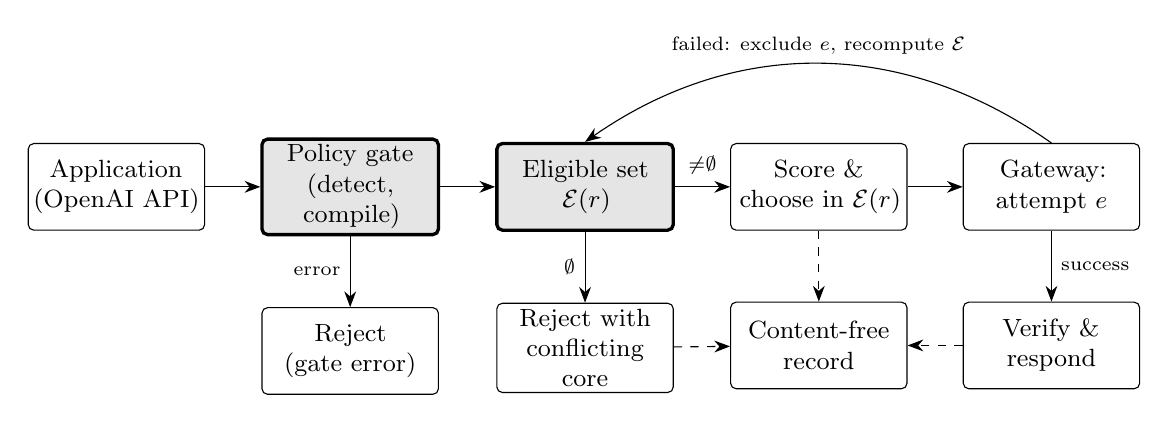
\begin{tikzpicture}[
  node distance=7mm,
  box/.style={draw, rounded corners=2pt, align=center, font=\small,
              minimum height=11mm, text width=21mm, inner sep=2pt},
  hl/.style={box, fill=black!10, very thick},
  arr/.style={-{Stealth[length=2mm]}}]
  \node[box] (app) {Application\\(OpenAI API)};
  \node[hl, right=of app] (gate) {Policy gate\\(detect, compile)};
  \node[hl, right=of gate] (elig) {Eligible set\\$\E(r)$};
  \node[box, right=of elig] (route) {Score \&\\choose in $\E(r)$};
  \node[box, right=of route] (gw) {Gateway:\\attempt $e$};
  \node[box, below=9mm of gate] (err) {Reject\\(gate error)};
  \node[box, below=9mm of elig] (rej) {Reject with\\conflicting core};
  \node[box, below=9mm of route] (rec) {Content-free\\record};
  \node[box, below=9mm of gw] (ver) {Verify \&\\respond};
  \draw[arr] (app) -- (gate);
  \draw[arr] (gate) -- (elig);
  \draw[arr] (gate) -- node[left, font=\scriptsize]{error} (err);
  \draw[arr] (elig) -- node[above=1pt, font=\scriptsize]{${\neq}\emptyset$} (route);
  \draw[arr] (route) -- (gw);
  \draw[arr] (elig) -- node[left, font=\scriptsize]{$\emptyset$} (rej);
  \draw[arr] (gw) -- node[right, font=\scriptsize]{success} (ver);
  \draw[arr] (gw.north) to[bend right=35] node[above, font=\scriptsize]{failed: exclude $e$,
    recompute $\E$} (elig.north);
  \draw[arr, dashed] (route) -- (rec);
  \draw[arr, dashed] (rej) -- (rec);
  \draw[arr, dashed] (ver) -- (rec);
\end{tikzpicture}
\caption{Request path. Eligibility is computed from the compiled policy and the endpoint
registry before any scoring; an empty set, or a gate error, rejects the request. A failed
attempt excludes that endpoint and recomputes the eligible set under the same execution
context. Every served, rejected or failed request writes one content-free record, including
its attempt chain, which the analyser of Section~\ref{sec:sim} replays. Optional context
compression, between the gate and the router, is omitted.}
\label{fig:pipeline}
\end{figure}

\paragraph{What an operator declares.} Per application: a placement, which is one
of \code{any}, \code{private\_cloud\_ok} or \code{onprem\_only}; allowed regions; whether a
provider may keep prompts; allowed tiers, providers and models; a per-request cost cap; and a
protection posture (Section~\ref{sec:eligibility}). Per endpoint: tier, price, region, prompt
retention, and whether it accepts unredacted sensitive text. RouteForge enforces policy against
these declarations. It cannot verify a provider's contractual claim, and an undeclared region or
retention never satisfies an application's requirement on it. (An endpoint whose acceptance of
unredacted sensitive text is undeclared is kept; only an explicit refusal excludes it.) When an
aggregator fronts several upstream providers, the declaration covers the aggregator endpoint as
a whole; RouteForge does not pin or observe the upstream provider.

\paragraph{The enforcement contract.} Write $E_{\mathrm{policy}}(r, \rho)$ for the endpoints
that satisfy request $r$'s compiled policy against registry state $\rho$, and
$\mathrm{Attempts}(r)$ for the endpoints the gateway sends $r$ to, in order. The property
RouteForge is designed to hold is
\begin{equation}
  \forall r,\ \forall e_j \in \mathrm{Attempts}(r):\quad e_j \in E_{\mathrm{policy}}(r, \rho_j),
  \label{eq:invariant}
\end{equation}
where $\rho_j$ is the registry state when attempt $j$ is selected. The execution context
(compiled policy, detected entity types, placement) is fixed once per request; eligibility is
\emph{recomputed} against current registry and configuration before every attempt, with
previously failed endpoints excluded. Exclusion only removes candidates, so a retry or failover
can never reach an endpoint the policy does not admit at that moment. An open circuit breaker
removes an endpoint from a tier's candidates, and when every candidate of the tier is open the
breaker is bypassed; the bypass restores only endpoints the policy had already admitted.

Equation~\eqref{eq:invariant} is a \emph{conditional design argument}, not a proof. It rests on
these assumptions: endpoint declarations in the registry are correct; application identity
(resolved from the bearer token) and policy loading are trusted; the detector inspects the
input it is given (text and tool-call arguments; RouteForge accepts no other modality); every
outbound inference call goes through the gateway; and the enforcement code itself is intact.
The argument is: eligibility is derived before selection; selection returns a member of the
eligible set or rejects; every retry and failover re-enters selection under the same execution
context; and no other component makes an inference call. The gateway records every attempted
endpoint, not only the one that served, so a denied attempt followed by a safe fallback would
be visible in the record as a violation. Section~\ref{sec:exp} checks
Eq.~\eqref{eq:invariant} on recorded attempt chains.

\paragraph{Trust boundary and external calls.} Table~\ref{tab:threat} lists which components
run inside the deployment, which make network calls, and what the paper does and does not
claim about each.

\begin{table}[t]
\centering
\small
\caption{Components, network behaviour and scope of the claim.}
\label{tab:threat}
\begin{tabular}{@{}p{3.4cm}p{5.0cm}p{6.3cm}@{}}
\toprule
component & network behaviour & scope \\
\midrule
PII detection & local (regex, or Presidio with a local spaCy model) & inside the boundary;
detector misses are out of scope (an undetected identifier is not restricted) \\
context compression & default compressor is local and offline; an optional third-party
compressor is opt-in & inside the boundary for the default; the optional compressor's internals
were not audited and it was off in every experiment \\
output verification & local, detector-based & inside the boundary; no LLM judge exists \\
inference, retry, failover & gateway only & subject to Eq.~\eqref{eq:invariant} \\
telemetry export & OTLP to a self-hosted Langfuse & redacted on export by default; raw capture
only for an application an operator opts in, to that application's own project \\
\midrule
malicious client & may choose its trajectory identifier & cannot choose its application
identity (token-derived); see Section~\ref{sec:envelope} \\
malformed policy & --- & each unparseable value resolves to its axis's protective end and the
write is refused \\
unavailable store & --- & the request is rejected (fail closed) \\
inaccurate endpoint declaration & --- & out of scope; enforced as declared, not verified \\
compromised trusted infrastructure & --- & out of scope \\
\bottomrule
\end{tabular}
\end{table}

\paragraph{The per-request cost cap is an estimated admission constraint.} It is not a spending
ceiling. At each selection the router estimates a candidate's cost from the input size (one
token per four characters of message text, plus serialised tools and tool calls) and an output
size (the client's \code{max\_completion\_tokens} or \code{max\_tokens}, else a configured
default of 512), priced at the endpoint's stated per-million-token rates without cache
discounts. A candidate whose estimate exceeds the cap is excluded. Every failover hop applies
the same cap to its own estimate; actual spend across the attempt chain is accounted after the
fact,
\[
C_{\mathrm{request}} = \sum_{j \in \mathrm{Attempts}(r)}
  \frac{p^{\mathrm{in}}_j n^{\mathrm{in}}_j + p^{\mathrm{out}}_j n^{\mathrm{out}}_j}{10^6},
\]
with $n$ the token counts the endpoint reports, but it is not enforced against the cap. Reasoning
tokens are billed as output; a failed attempt that returns no usage contributes zero. Section~\ref{sec:tokens}
reports how far the estimate departs from the serving engine's count.

\paragraph{The router.} The target tier is a function of request length,
$\mathit{complexity} = \min(1, \mathit{tokens}/2000)$, with thresholds 0.35 and 0.70 separating
the cheap, mid and frontier tiers; it is not a semantic estimate. The target is raised to the
request's risk floor and the application's minimum tier, and lowered to the best tier the
application allows. If the target tier has no eligible endpoint the router moves up to the
next tier that has one. If nothing in that tier fits the cost cap it steps down to the most
capable cheaper tier that does, never below the risk floor; if none fits, the request is
rejected. Among the eligible endpoints of the chosen tier it maximises
\begin{equation}
  w_q\, q \;-\; w_c\, \frac{c}{c_{\max}} \;-\; w_l \min\!\left(\frac{\ell}{s}, \kappa\right)
  \;+\; w_a\, a ,
  \label{eq:score}
\end{equation}
where $c$ is the candidate's estimated request cost in USD and $c_{\max}$ the largest such
estimate among the candidates being scored (so the normaliser changes with the candidate set;
the term is 0 if $c_{\max}=0$); $\ell$ is latency in ms, scaled by $s = 1000$\,ms and capped at
$\kappa = 3$; $a \in [0,1]$ is availability; and $q \in [0,1]$ is quality. The shipped weights
are $w_q, w_c, w_l, w_a = 1.0, 0.6, 0.3, 0.2$. Latency and availability are moving averages of
the gateway's own calls to the endpoint; without enough recent samples, latency falls back to
a same-tier peer's measurement or a default for the tier, and availability to a neutral 1.
Quality is a score the operator supplied, a calibrated or published score, or otherwise a
default for the tier (0.5, 0.75, 1.0). Ties are broken by lower estimated cost, then by
registry order. Each term is recorded with its value and where that value came from, so a
ranking can be recomputed offline.

\paragraph{What is recorded.} Every request writes one content-free record: application,
detected entity \emph{types}, placement, target tier, the eligible set, each rejected endpoint
with a reason code, the attempt chain, the chosen endpoint, a status (served, rejected, failed),
token counts, cost, latency, and the versions of the application policy, the endpoint registry
and the routing configuration. It contains no prompt or completion text. ``Content-free'' does
not mean anonymous: application identifiers, timestamps, token lengths and entity types remain
potentially sensitive metadata.

% ---------------------------------------------------------------------------
\section{Eligibility, placement and protection}
\label{sec:eligibility}

\paragraph{Two kinds of axis.} \emph{Placement} governs where compute may run. \emph{Protection}
governs what the model is shown, what the client receives, what telemetry stores, which
detector runs, and whether lossy transformations and streaming are allowed. Table~\ref{tab:axes}
enumerates the axes.

\begin{table}[t]
\centering
\small
\caption{Policy axes. ``Protective end'' is the value an unparseable input resolves to; such a
write is also refused. Placement axes change endpoint eligibility; protection axes change data
handling and never eligibility.}
\label{tab:axes}
\begin{tabular}{@{}lp{5.2cm}p{2.6cm}l@{}}
\toprule
axis & values (stricter to the right or by inclusion) & protective end & kind \\
\midrule
residency & \code{any} $<$ \code{private\_cloud\_ok} $<$ \code{onprem\_only} & \code{onprem\_only} & placement \\
allowed regions & a set of region labels; $R' \subseteq R$ is stricter; unset = no constraint & empty set & placement \\
no retention & false $<$ true & --- & placement \\
allowed tiers / providers / models & sets, ordered by inclusion & --- & placement \\
cost cap (USD) & a number; lower is stricter & --- & placement \\
\midrule
model input & \code{raw} $<$ \code{redact} & \code{redact} & protection \\
client output & \code{raw} $<$ \code{redact} & \code{redact} & protection \\
telemetry I/O & \code{full}, \code{redacted}, \code{off} & \code{off} & protection \\
detection & \code{off}, \code{regex}, \code{presidio} & \code{presidio} & protection \\
content integrity & \code{transformations\_allowed} $<$ \code{exact} & \code{exact} & protection \\
stream mode & \code{off} and three opt-in modes & \code{off} & protection \\
\bottomrule
\end{tabular}
\end{table}

\paragraph{Resolution and ceilings.} Each optional setting is resolved by precedence: the
application's explicit value, then a preset (\code{enforced} or \code{passthrough}), then the
deployment default. A deployment \emph{ceiling} is then applied as a clamp, not as one more
level of precedence: if the deployment does not permit passthrough, or does not permit an
application to weaken detection, an explicit application value of \code{raw} becomes
\code{redact}, and \code{off} or \code{regex} detection becomes the deployment's detector, even
though the application's value would otherwise win. A missing or non-boolean ceiling flag
denies. For example, an application that sets \code{model\_input: raw} on a deployment whose
ceiling forbids passthrough compiles to \code{model\_input: redact}, and the compiled policy
records that the value was clamped. Placement has no ceiling flag; it can only be tightened,
by the application or by a sensitivity rule.

\paragraph{Compiler component independence.} We use a restricted, static form of
noninterference~\cite{goguen}. The policy is compiled in two stages, and each property holds
with the other stage's inputs fixed:
\begin{enumerate}
  \item \emph{Static compilation} resolves placement and protection from configuration. Writing
    $\mathrm{place}(\cdot)$ and $\mathrm{prot}_b(\cdot)$ for the placement and protection
    components of the compiled policy:
    \begin{description}
      \item[NI-1.] For any policy $\pi$, protection axis $a$, values $v, v'$, and a fixed tuple
        of detected entity types:
        $\mathrm{place}(\mathrm{compile}(\pi[a{=}v])) = \mathrm{place}(\mathrm{compile}(\pi[a{=}v']))$.
      \item[NI-2.] For placement values $p, p'$ and every protection axis $b$:
        $\mathrm{prot}_b(\mathrm{compile}(\pi[\mathrm{place}{=}p])) =
         \mathrm{prot}_b(\mathrm{compile}(\pi[\mathrm{place}{=}p']))$.
    \end{description}
  \item \emph{Sensitivity rules} are then applied to the observed entity types. A rule may only
    raise placement (and may set a sensitivity label and require output verification, neither
    of which is a protection axis), and every rule that fires is named on the response and
    the record.
\end{enumerate}
NI-1 holds the observation fixed. It does not say that changing the detector leaves runtime
placement unchanged for the same text: switching detection from \code{presidio} to \code{off}
changes what is observed, and so, through stage~2, what placement the request receives. That
interaction is declared and raise-only, but it exists, and NI-1 is not a claim about final
routing.

\paragraph{Eligibility and monotonicity.} Given the compiled policy and the endpoint registry,
the eligible set is computed in one place. For fixed request features and registry, if
$\pi'$ is stricter than $\pi$ on every axis of Table~\ref{tab:axes}, then
\[
  E_{\mathrm{policy}}(r, \pi') \subseteq E_{\mathrm{policy}}(r, \pi).
\]
This does not extend to the router's served/rejected decision: the tier, risk-floor and budget
logic above can reject a request whose eligible set is nonempty, and Section~\ref{sec:neg}
gives a case where \emph{relaxing} placement makes a request newly rejected. We therefore keep
two kinds of rejection apart: \emph{policy infeasibility} ($\E$ is empty) and \emph{router
refusal} ($\E$ is nonempty but no candidate fits the cost cap at or above the risk floor).

\paragraph{Checking it.} Eight invariants are stated as ten property functions over generated
policies and registries (200 examples by default, 2{,}000 in a deeper profile), using
property-based testing~\cite{quickcheck,hypothesis}. On its first run the harness found two
fail-open defects in shipped code. An empty placement string compiled to \code{any} through a
default-on-falsy idiom. And two code paths each decided placement: the compiler said
\code{onprem\_only} while the request context still listed two cloud providers; the fix was a
single authority. Both are kept as regression fixtures. Against 18 hand-written single-edit
mutants of the compiler, each targeting the behaviour one property asserts over, the harness
catches 15 (83\%). The three survivors are: an equivalent mutant (a bypassed membership check
that falls through to a second guard which is itself covered); a mutant of a redundant
normalisation that an earlier stage already performs, so no property can observe it; and a
guard on malformed deployment defaults that the generators could not reach, because they drew
only legal defaults. The last was a coverage gap, not an equivalent mutant; the generators now
draw malformed defaults and three mutants on that path are caught. A mutation score measured
against generators that cannot reach the mutated line overstates adequacy, and the overstatement
looks exactly like an equivalent mutant. The mutants were written by the author of the
properties and are not independent of them. The mutant list, generators and seeds are in the
artifact (Section~\ref{sec:artifact}).

\paragraph{Explaining a rejection.} When $\E$ is empty, each endpoint fails a set of
requirements. A \emph{conflicting core} is a set of requirements that together exclude every
endpoint, i.e.\ a hitting set of the endpoints' failure sets. RouteForge returns a
\emph{minimum-cardinality} core, found exactly by searching subsets in increasing size over at
most eleven requirement identifiers ($2^{11}$ subsets); ties are broken by a fixed requirement
order. A minimum core is also subset-minimal. For example, with two endpoints, an on-premises
endpoint that fails \{\code{allowed\_regions}, \code{max\_cost}\} and a cloud endpoint that fails
\{\code{residency}, \code{no\_retention}\}, every core needs one requirement from each, so a
minimum core has size two, and the fixed order selects \{\code{residency},
\code{allowed\_regions}\}. The failure sets are computed once, for the request's fixed context;
the core is not re-validated by relaxing its members and recomputing derived predicates.
Endpoint \emph{state} (no endpoints configured, disabled, breaker open, already failed in this
request) is reported separately and is never part of a core, so ``nothing is onboarded'' is not
confused with contradictory policy. No remediation hint proposes relaxing a security
requirement. The search's runtime at eleven requirements was not measured.

% ---------------------------------------------------------------------------
\section{Evaluating a router that has to obey a policy}
\label{sec:eval}

For a case $c$ with eligible set $\E(c)$, quality $q(c,e)$ and a quality floor $f(c)$:
\begin{align*}
  q^*(c) &= \max_{e \in \E(c)} q(c,e), &
  P(c) &= \{\, e \in \E(c) : q(c,e) \ge f(c) \,\}.
\end{align*}
The cost oracle is the cheapest endpoint in $P(c)$ and the latency oracle the fastest; they
can be different endpoints and are separate lower bounds. If $\E(c)$ is empty the correct
outcome is a rejection, and a strategy is scored on whether it rejects. If $\E(c)$ is nonempty
but $P(c)$ is empty, quality regret is defined against $q^*(c)$ and no cost or latency oracle
exists. A call that an endpoint refused or that timed out is an endpoint failure, reported
separately from a wrong answer, never as quality zero. In live runs, cost and latency are the
measured values of each call; in simulation they come from declared prices and latency
profiles.

FeasibleRouteBench reports, for each routing strategy: the \textbf{violation rate} (a choice
outside $\E(c)$, which fails the run), pass rate and quality regret, cost and latency regret,
and correct handling of empty-set cases. The oracle never credits an endpoint outside $\E(c)$.
Cost and latency regret are computed over the cases a strategy passed, which can favour a
strategy that fails hard cases; pass rate and case counts are always reported beside them,
and in the live benchmark below every strategy passed every answered case, so the comparison is
over common cases. Results are also reported per group of cases (placement, protection,
application, workload) with the case count beside every figure, and no figure for a group below
a minimum size.

\paragraph{An offline version check (experimental).} A candidate routing configuration is
scored beside the current one on the same cases, the paired per-case difference of each named
metric is bootstrapped over cases~\cite{efron} (1{,}000 resamples by default, 90\% two-sided
percentile interval), and each \emph{figure}---one metric, overall or within one group---is
judged on its whole range: \code{regressed} if the entire range lies beyond the tolerance in
the worsening direction, \code{within tolerance} if it lies entirely inside, and
\code{inconclusive} otherwise. A candidate's verdict is \code{regressed} if any judged figure
is. No correction is made for the number of figures judged.

We measured the false-alarm rate of this candidate-level verdict in a synthetic null
experiment: two arms scored from one shared distribution, so there is no true difference, with
a share $f$ of the 22 cases redrawn between the arms (modelling fresh stochastic generations or
noisy endpoint measurements; on an identical frozen matrix every paired difference would be
zero and no figure could regress), 300 draws per setting and 400 resamples. With nonzero
tolerances on one or two metrics (14 to 28 figures judged), an earlier rule that judged the
point estimate called the candidate regressed in 66\% to 97\% of draws; the whole-range rule
does so in 0.3\% to 31\%: about 2\% and 0.3\% with $f = 0.3$, and 25\% to 31\% with every case
redrawn. With all eight metrics at zero tolerance (102 to 108 figures) the rates are 100\% and
55\% to 83\%. A false-alarm rate of a quarter to a third, when every case is redrawn, is too
high for a promotion gate. We therefore present the check as experimental: its
\code{regressed} verdict has no controlled error rate, a family-wise correction is not built,
and the script for this null experiment is not in the repository. The check applies nothing;
a routing change is still made by an operator.

\paragraph{Failure injection.} In simulation, where quality is an input, the harness is
exercised with failure injection. From Eq.~\eqref{eq:score} follows a condition for when a dead
endpoint (availability $a$) loses the ranking to a same-tier peer, under these assumptions: the
two have equal quality and equal latency contribution, the peer's availability is 1, the
peer's estimate is the largest in the candidate set so that $c_{\max}$ is the peer's cost, and
$p<1$ is the dead endpoint's price relative to the peer. It loses only if
$w_a (1 - a) > w_c (1 - p)$. At the shipped weights a fully dead endpoint ($a = 0$) cheaper than
two thirds of its peer's price still ranks first, which motivated a circuit breaker.

% ---------------------------------------------------------------------------
\section{Predicting the effect of a policy change}
\label{sec:sim}

\paragraph{Replay.} The analyser reads an export of outcome records and a configuration
snapshot, and runs each record's first routing decision through the production context
builder, eligibility function and router twice: under the current configuration and under a
proposal. The reported effect is the difference between the two simulated arms. Agreement
between the current arm and what was recorded is a fidelity check, reported with every result
and usable as a gate.

Because the records were produced by a deterministic router, they contain no overlap between
policies, and off-policy estimators~\cite{bottou,dudik} do not apply. Replay is possible only
because routing is a pure function of recorded inputs.

\paragraph{What kind of counterfactual.} Separate policy eligibility from operational readiness:
\[
  E_{\mathrm{dispatch}}(r,t) = E_{\mathrm{policy}}(r) \cap H(t),
\]
where $H(t)$ is the set of endpoints that are not disabled and whose breakers are not open at
time $t$ (with the bypass of Section~\ref{sec:system} as an operational exception, never an
exception to $E_{\mathrm{policy}}$). Replay evaluates the first decision with \emph{frozen
latency and availability signals} from the snapshot and assumes $H(t)$ contains every enabled
endpoint: it is replay of a healthy deployment. It does not replay retries or failover, breaker
state, or the health evolution a different allocation would cause. Its strongest claims are
deterministic changes in eligibility and selection from logged inputs. Cost, latency and
quality figures for endpoints that did not serve a request are estimates from the snapshot's
prices and profiles, not measured outcomes; replay does not say what an alternative model would
have answered or how long its answer would have been.

\paragraph{Supported scenarios.} Table~\ref{tab:supported} states which proposals content-free
records can and cannot evaluate. These are limits of the method; the analyser excludes records
that lack required features, but it does not detect every unidentifiable proposal, so the
operator must.

\begin{table}[t]
\centering
\small
\caption{Proposals that replay over content-free records can and cannot evaluate.}
\label{tab:supported}
\begin{tabular}{@{}p{7.2cm}p{7.4cm}@{}}
\toprule
supported & not identifiable from the records \\
\midrule
change an application's placement, regions, retention, tier/provider/model allowlists or cost
cap & a new or changed detector, or a detector threshold (entities never detected were never
recorded) \\
change sensitivity rules over \emph{recorded} entity types & a new semantic feature of the
prompt \\
change routing weights, thresholds or prices & what an alternative endpoint would have answered,
or its output length \\
onboard, disable or redeclare an endpoint (with a stated profile) & queueing and latency under
a different traffic allocation \\
stated-capacity utilisation per endpoint & concurrency (records do not hold active intervals) \\
\bottomrule
\end{tabular}
\end{table}

\paragraph{Scenarios.} Several proposals are compared side by side against one shared current
arm: routes changed, requests newly rejected and newly served, and the change in stated cost,
latency, quality and on-premises share. The report lists scenarios in file order and never
ranks them. Cost differences are computed only over requests routed in both arms; a newly
rejected request is never counted as a saving.

\paragraph{The price of a requirement.} For one application and one requirement, relax it,
replay, and difference. The result is an empirical price on the recorded traffic, not a dual
variable. For a security requirement it is labelled ``price of a protection---not a
recommendation''.

\paragraph{Uncertainty.} For a fixed export, the number of changed routes is deterministic.
Each difference additionally carries a 90\% percentile range from a paired bootstrap of the
replayed records, stratified by application. Its estimand is the expected difference for a
workload of the same size drawn from the same process as the export, under the assumption that
records are independent; it is a confidence interval for that expectation, not a prediction
interval for the next run's realised count. The independence assumption fits our synthetic
generator, which draws each request independently. It does not fit agent sessions, where the
resampling unit should be the session or task, nor minute-level peaks, where a row bootstrap
destroys the bursts that matter. A count of zero is printed with a one-sided bound on its
rate, not as zero risk.

\paragraph{Capacity.} An operator states limits per endpoint (concurrency, requests and tokens
per minute). Replayed demand in each arm is bucketed in time and compared with the stated
limits, reporting the peak, the time-average and the share of buckets over the limit, always
with the bucket length. It reads stated limits only: it does not predict queueing, and per-minute
counts cannot establish concurrency without request durations.

% ---------------------------------------------------------------------------
\section{Experiments}
\label{sec:exp}

\subsection{Setup}

All live runs are on one GPU lab running production builds of RouteForge
(Table~\ref{tab:endpoints}). On-premises prices are illustrative values the operator declared.
Cloud prices are the aggregator's paid list prices for the same models, read on 2026-10-09; the
free variants actually called were billed nothing. \textbf{Every dollar figure in this section
is stated-price accounting, not a bill.}

\begin{table}[t]
\centering
\small
\caption{Endpoints in runs 3 and 4. Prices are stated, in USD per million input/output tokens.
On-premises endpoints are OpenAI-compatible servers on the lab's H200 GPUs; cloud endpoints are
free variants reached through the OpenRouter aggregator.}
\label{tab:endpoints}
\begin{tabular}{@{}p{6.3cm}llll@{}}
\toprule
endpoint (model identifier) & provider & tier & price in/out & retention \\
\midrule
\code{Qwen3.6-35B-A3B}, FP8, one H200 & on-premises & cheap & 1 / 1 & none \\
\code{zai-org/GLM-5.3-Flash} & on-premises & mid & 10 / 10 & none \\
\code{nvidia/nemotron-3-super-}\newline\code{\quad 120b-a12b:free} & cloud & mid & 0.08 / 0.45 & retained \\
\code{nvidia/nemotron-3-ultra-}\newline\code{\quad 550b-a55b:free} & cloud & frontier & 0.50 / 2.20 & retained \\
\bottomrule
\end{tabular}
\end{table}

The cloud endpoints are declared as retaining prompts and as refusing unredacted sensitive
text, because RouteForge cannot verify what an upstream provider keeps. The on-premises models'
serving-engine versions, launch settings and weight revisions were not recorded with the runs;
the endpoint declarations are in each run's configuration snapshot.

Three applications: \emph{claims} (per-request cap \$0.05), \emph{dev}, and \emph{clinic}
(on-premises only, one allowed region, no retention). Traffic is synthetic: each request is
drawn independently (application; kind of text among prose, code, logs and JSON; a
heavy-tailed length; and with some probability a planted SSN and e-mail address). Runs 1 and 2
used one model; runs 3 and 4 used the four endpoints of Table~\ref{tab:endpoints}
(Table~\ref{tab:runs}). Every request ends in one of three statuses: \emph{served},
\emph{rejected} (policy infeasibility or router refusal), or \emph{failed} (admitted, but every
attempt failed).

\begin{table}[t]
\centering
\small
\caption{Live runs. Statuses are served / rejected / failed.}
\label{tab:runs}
\begin{tabular}{@{}cp{3.4cm}rp{2.6cm}p{5.0cm}@{}}
\toprule
run & endpoints & rows & statuses & what it adds \\
\midrule
1 & one on-premises model & 912 & --- & replay baseline; range behaviour \\
2 & one model under three declared names & 900 & 880 / 18 / 2 & declarations; a designed 181.5\,s outage \\
3 & four models & 899 & 878 / 21 / 0 & cloud path; the provider's quota ran out after 6 of 30 minutes \\
4 & four models & 900 & 878 / 22 / 0 & cloud path working throughout \\
\bottomrule
\end{tabular}
\end{table}

\subsection{Placement holds}

In runs 3 and 4, 641 rows belonged to the on-premises-only application and 346 rows from the
other two applications were raised to on-premises placement because an entity was detected.
\textbf{None of the 987 had a cloud endpoint anywhere in its recorded attempt chain}, including
retries and failovers. These are requests restricted by the compiled policy, not every truly
sensitive request that could occur. Under independent Bernoulli trials, zero violations in 987
gives a one-sided 95\% upper bound on the violation rate of $1 - 0.05^{1/987} \approx 0.30\%$;
for a deterministic program this is a description of the sample, not a security bound over
unseen policies, which is what the property checks of Section~\ref{sec:eligibility} address. A
request from the on-premises-only application that names a cloud model is refused with the
reason. In every benchmark run, simulated and live, no strategy chose an endpoint outside a
case's eligible set.

A pattern detector has a cost here that is easy to miss. In run 4, 83 of the 173
detection-raised requests (48\%) carried no planted identifier: random digits in synthetic logs
and JSON matched credit-card and bank-number patterns. This is the share of a selected group,
not the detector's false-positive rate, which needs the count of truly negative requests; we
have not computed a confusion matrix against the generator's ground truth, nor the false-negative
rate. The errors observed are in the safe direction---those requests stayed on-premises---and
they are paid for at the on-premises price.

\subsection{Replay fidelity}

\begin{table}[t]
\centering
\small
\caption{Replay fidelity: agreement of the replayed current arm with what was recorded.
\emph{Admission} compares the first routing decision, routed or rejected, over all rows (a
failed request was routed); \emph{first endpoint} compares the replayed first choice with the
endpoint that served, over served rows. Attempt-chain and
cost agreement are not reported because replay is first-decision only.}
\label{tab:fidelity}
\begin{tabular}{@{}clll@{}}
\toprule
run & endpoints during the run & admission agreement & first-endpoint agreement \\
\midrule
1 & answering & 1.0 over 912 & 1.0 \\
2 & one endpoint down for 181.5\,s & 1.0 over 900 & 0.926 over 880 \\
3 & cloud provider down for 24 of 30 min & 1.0 over 899 & 0.919 over 878 \\
4 & answering (one endpoint refusing a third of calls) & 1.0 over 900 & 1.0 over 878 \\
\bottomrule
\end{tabular}
\end{table}

Replay matched the recorded first-decision admission of all 3{,}611 rows
(Table~\ref{tab:fidelity}): every request recorded as rejected replayed as rejected, and every
request recorded as served or failed replayed as routed. Admission agreement does not test
whether a routed request would be served; the two failed requests of run 2 count as routed in
both arms. Endpoint
identity agreed completely when endpoints were answering and diverged during outages. In run 2
all 65 disagreements were requests the live router diverted because a breaker was open. In run
3 replay sent 180 requests to a provider that answered 31, and its baseline cost was 26\% below
the recorded cost; in run 4 the two costs were within 1.2\%. \textbf{Replay describes the
deployment with its endpoints healthy.} It does not model breaker or failure state, and its
figures should be read that way.

Fidelity also depends on recording every input the router reads. An early deployment did not
record a client's explicit model choice; replay agreement was 0.0206 over 194 rows, behind a
report that looked plausible. After recording it, agreement was 1.0. Similarly, rejected
requests once recorded a token count of zero and replayed as served (7 of 7) until the router's
own token count was recorded on every row.

\subsection{What a policy change costs}

\begin{table}[t]
\centering
\small
\caption{Policy scenarios replayed over run 4 (900 rows; replayed baseline \$7.02, stated
prices). Ranges are 90\% paired-bootstrap intervals for the expected difference.}
\label{tab:scenarios}
\begin{tabular}{@{}p{6.2cm}lll@{}}
\toprule
proposal & routes changed & newly rejected & $\Delta$ cost, \$ \\
\midrule
on-premises only for \emph{claims} and \emph{dev} & 178 [160, 197] & 0 & +3.74 [3.20, 4.30] \\
``no prompt retention'' for \emph{claims} and \emph{dev} & 178 [160, 197] & 0 & +3.74 [3.20, 4.30] \\
let \emph{clinic} use the cloud & 63 [52, 75] & 0 & $-$0.89 [$-$1.19, $-$0.65] \\
raise the per-request cap tenfold & 15 [9, 22] & 0 (22 newly served) & +0.76 [0.46, 1.15] \\
\bottomrule
\end{tabular}
\end{table}

Two different requirements---a placement and a retention rule---produce the same 178 moves
(Table~\ref{tab:scenarios}), because the cloud endpoints are declared as retaining prompts; the
report shows each under its own name. Run 3 gave +\$3.12 [2.69, 3.54] for the first proposal on
a separate sample; the ranges overlap.

\paragraph{A prediction followed by a measurement.} Run 3's replay was computed while the cloud
provider was refusing every call, and put 180 requests [163, 199] on the cloud under the current
policy. Run 4, an independent draw from the same generator with the provider answering, recorded
178. This is one agreement, on synthetic traffic; it does not establish the calibration of the
ranges or predictive accuracy in general.

\paragraph{A static check can call a tightening free when it is not.} In run 2, restricting two
applications to one region left another endpoint eligible for every application, so a check of
the configuration alone finds nothing lost. Replay found 5 requests [2, 9] rejected, because the
remaining endpoint was over those requests' budget; a retention rule likewise rejected 4 [1, 7].
In runs 3 and 4, with an inexpensive on-premises endpoint available, the same kind of tightening
rejected none. The effect depends on what else is eligible for the traffic that actually
arrives, which is the argument for replay over inspection.

\paragraph{Capacity.} In run 4, moving everything on-premises takes the on-premises mid endpoint
from 50.0\% to 90.9\% of its stated requests-per-minute limit in its busiest minute
(time-average 30.3\% to 41.1\%), a consequence the cost table does not show.

\paragraph{Ranges.} On run 1's 912 independent rows the width of a range shrinks roughly as
$1/\sqrt{n}$ from $n = 200$. Splitting the export in half 100 times, the range from one half
contained the other half's point estimate 66\% to 76\% of the time, against a reference of 75.5\%
for a calibrated 90\% range of a difference between two independent halves. Both are
diagnostics; coverage against a known truth has not been measured, nor under the dependence of
agent-loop traffic.

\subsection{The router's choices, on a benchmark}
\label{sec:bench}

We use two suites. The \emph{starter} suite has 22 short cases. The \emph{extended} suite is
generated (seed 20261009): 6 policy groups $\times$ 6 workloads $\times$ 3 length bands $=$ 108
cases. The six policy groups are five placement \emph{scenarios}---\code{any} (with an
\code{enforced} and a \code{passthrough} variant, 18 cases each), \code{onprem\_only},
\code{us\_only} (\code{any} with one allowed region), \code{no\_retention} (\code{any} with no
retention) and \code{escalated} (\code{any} with a planted SSN that raises placement), 18 cases
each---so the five scenarios are not the three values of the residency axis, and the two
protections are unbalanced (90 enforced, 18 passthrough). The six workloads (arithmetic,
extraction, JSON, classification, reading, code) have 18 cases each, and the three length bands,
which target the cheap, mid and frontier tier under the length rule, 36 each. Every case is
answerable from its own text. One call per case and eligible endpoint (252 calls a sample), a
deterministic grader, no retries, and three samples (756 calls).

\paragraph{Quality.} Of 756 calls, 18 errored (15 on the free cloud frontier endpoint:
overload, API errors and two rate limits; three HTTP 500s on-premises) and are reported as
endpoint failures. Every answered call passed: 738 of 738. The suite is at ceiling and cannot
rank the models; it is an equal-quality cost stress test, not evidence of routing
effectiveness. An earlier run on the starter suite had the cheap model passing 18 and 19 of 22
cases against the mid model's 16, which invites the reading that the tier order is wrong for
this pair. \textbf{We do not make that claim.} The starter suite contains cases that cannot be
answered from their prompt, and the gap did not survive well-posed cases. What the two suites
support together is narrower: a tier is not a quality measurement, and a small suite with
strict graders can manufacture a ranking.

\paragraph{Cost at equal quality.} Because every endpoint passed every answered case, the
cheapest eligible endpoint is the oracle, and the router's regret is pure stated cost
(Table~\ref{tab:regret}).

\begin{table}[t]
\centering
\small
\caption{Extended suite, cost at equal quality: mean stated cost per case, USD.}
\label{tab:regret}
\begin{tabular}{@{}lccc@{}}
\toprule
sample & cheapest eligible & RouteForge router & ratio \\
\midrule
1 & 0.000883 & 0.005925 & 6.71 \\
2 & 0.000873 & 0.005957 & 6.83 \\
3 & 0.000877 & 0.005924 & 6.75 \\
\bottomrule
\end{tabular}
\end{table}

The router pays about 6.7 to 6.8 times the cheapest eligible price for the same result, with a
cost regret of about \$0.0050 per case; both strategies passed every answered case. The cause is
the length-based tier rule: a longer request targets a higher tier whether or not it is harder.
Two thirds of this suite is long by construction and the prices are stated, so the ratio is a
property of the suite; the direction is a property of the rule. No strategy chose an endpoint
outside a case's eligible set in any run.

Where two endpoints shared a tier and a quality default in live traffic, the cost term decided:
all 84 unrestricted mid-tier requests in run 4 went to the cloud endpoint.

\paragraph{The version check on live endpoints.} On the starter suite, two candidates that
changed scoring weights altered no route and passed trivially; a candidate that removes the
cheap tier changed 12 of 22 routes and was \code{inconclusive}. On the extended suite the same
candidate changed 30 of 108 routes and raised mean chosen cost by \$0.00014 per case, with a 90\%
range of [0.000085, 0.00020] that excludes zero. The tolerance had been set in advance at
0.0005, the whole range lies inside it, and the verdict was \code{pass}: a real worsening,
measured, and smaller than what we had said we would accept. All 38 judged figures had enough
cases. Separately from the 18 compiler mutants of Section~\ref{sec:eligibility}, the check
catches 15 of 15 single-rule mutations of its own detectors in simulation, and flags planted
regressions. A \code{regressed} verdict on live endpoints has not been produced.

\subsection{Failures}

\begin{table}[t]
\centering
\small
\caption{Failures in the live runs.}
\label{tab:failures}
\begin{tabular}{@{}lp{3.6cm}p{3.6cm}p{3.6cm}@{}}
\toprule
 & run 2 & run 3 & run 4 \\
\midrule
cause & one endpoint refused for 181.5\,s & cloud quota exhausted for 24 min & one cloud endpoint refused 35 of 94 calls \\
requests failed & 2 of 900 & 0 of 899 & 0 of 900 \\
wasted attempts & 8 on the dead endpoint & 102 & 35 \\
\bottomrule
\end{tabular}
\end{table}

Table~\ref{tab:failures} summarises the outages.
\begin{itemize}
  \item When the failing endpoint shared its tier with a healthy one, the breaker removed it
    with no wasted call: 71 of 89 such requests in run 3.
  \item When it was alone in its tier, the breaker was bypassed, by design, so that an open
    breaker alone never refuses a request. With lower tiers available this costs one failed call
    per request and buys nothing: 79 of run 3's 102 wasted attempts.
  \item Failover moved requests \emph{down} a tier: 13 frontier-target requests were served by
    the cheap endpoint in run 3, and 35 by the mid endpoint in run 4. Nothing on the record marks
    this except comparing the target tier with the endpoint that served.
  \item The two failures in run 2 were requests for which the budget left one affordable
    endpoint, and that endpoint was down.
\end{itemize}

\paragraph{Stated capacity against behaviour.} The cloud provider publishes 20 requests a minute.
In run 3 replayed demand peaked at 30\% of that while every call was refused: the binding limit
was a daily allowance. In run 4 neither cloud endpoint passed 45\% and one refused 37\% of calls
as overloaded. The capacity reading is only as good as the limits stated, and here they were not
the limits that bound; daily quotas, burst controls and provider overload are outside it.

\subsection{Two measurements about tokens}
\label{sec:tokens}

\begin{itemize}
  \item \textbf{The admission estimate depends on the kind of text.} RouteForge sizes a request
    at one token per four characters. Against the serving engine's count on run 1, the ratio was
    1.72 on prose, 0.79 on code, 0.70 on JSON and 0.52 on log lines, and 0.955 summed---an
    aggregate that hides a threefold spread. On the 21 served calls of a real coding agent
    session it was 0.96 to 1.02. A per-request cap enforced on this estimate over-rejects prose
    and under-counts logs; it is an admission heuristic, not a bound on spend.
  \item \textbf{HTTP success is not a useful answer.} Both on-premises models reason before
    answering, and reasoning is billed as output. With output limits of 768 to 1{,}536 tokens,
    43\% of the cheap model's answers and 20\% of the mid model's in run 4 had no visible text.
    Each is an HTTP 200 with a full bill, and the record does not distinguish it from a useful
    answer; the synthetic traffic requested no tool calls, so these are not tool-only replies.
    We did not separate finish reasons, truncation and reasoning-only responses, and we read the
    rates as a sensitivity to the output-limit configuration on this synthetic traffic, not as a
    property of the models.
\end{itemize}

% ---------------------------------------------------------------------------
\section{Negative results and limits}
\label{sec:neg}

\paragraph{The router is not monotone in the eligible set.} Eligibility is monotone: relaxing a
requirement never removes an endpoint. The router is not: with a placement clamp and a budget
fallback that respects a risk floor, relaxing placement for a request with a tight budget and a
detected identifier can make it newly rejected as over budget. We have a constructed example and
a test that pins it. It did not occur in 2{,}699 live rows across three runs, in which every
relaxation newly rejected nothing. The only invariant a relaxation satisfies is that the
eligible set grows.

\paragraph{A scoring term can be inert.} One term of the scoring rule was, for the product's
history to that point, algebraically unable to change a ranking; a weight of 0.2 or 20 gave
identical outcomes. Recording each term's value and source per decision is what exposed it.

\paragraph{The router does not choose well among eligible models} (Section~\ref{sec:bench}). Tier
is a function of length, and quality is a default unless measured. On a benchmark at ceiling it
paid about 6.7 times the cheapest eligible stated price for the same answers.

\paragraph{A small suite can manufacture a ranking.} Our first benchmark runs suggested the cheap
model was better than the mid one. A larger suite of well-posed cases removed the gap. We report
the episode because the first reading was ours, and it was wrong.

\paragraph{Not measured.} A saving against a frontier-only baseline: the lab has no paid prices.
Any difference in quality between the models: the larger suite is at ceiling. A baseline that
applies the same eligibility predicates through a generic policy engine before the same scoring
rule. Gate, compilation, eligibility and replay overhead, and the conflicting-core search time.
Attempt-chain agreement under replay. A detector confusion matrix. A \code{regressed} verdict
from the version check on live endpoints, and a controlled false-alarm rate for it. Coverage of
the uncertainty ranges, directly or under dependence. Any effect on real text: every prompt in
Section~\ref{sec:exp} is synthetic, except the content-free records of one coding-agent session
(40 rows, of which 21 were served and 19 rejected by the cost cap).

\paragraph{Other threats.} One deployment; each outage is a single event; run 2's three
endpoints were one model under three declarations; endpoint declarations are the operator's and
are not verified; the benchmarks are synthetic single-turn cases with deterministic graders; the
version check makes no correction for the number of figures it judges; replay is first-decision
with frozen signals; the live runs span several builds of RouteForge (Section~\ref{sec:artifact}).

% ---------------------------------------------------------------------------
\section{From request-level to trajectory-level feasibility}
\label{sec:traj}

Everything above treats a request as the unit. An agent does not make a request; it makes a
\emph{trajectory}: tens of related calls while it plans, calls tools, reads results, retries and
resumes. By default RouteForge sees each call separately and keeps no state between them. Two
observations show what that leaves out (Sections~\ref{sec:compaction} and~\ref{sec:resend}). We
then state the problem (Section~\ref{sec:trajproblem}) and report a prototype for its placement
part (Section~\ref{sec:envelope}). Cache-aware optimisation, quality-aware sequential routing and
feasible-trajectory regret are not implemented.

\subsection{A restriction that does not survive compaction}
\label{sec:compaction}

One conversation from an application with unrestricted placement, run three times on the lab of
Table~\ref{tab:endpoints}, with synthetic text (Table~\ref{tab:compaction}).

\begin{table}[t]
\centering
\small
\caption{A three-turn conversation, three runs, no envelope.}
\label{tab:compaction}
\begin{tabular}{@{}lp{8.2cm}l@{}}
\toprule
turn & what the client sent & served by (3 runs) \\
\midrule
T1 & a public question & cloud, cloud, cloud \\
T2 & T1 plus a tool result containing an SSN and an e-mail address & on-premises $\times 3$ \\
T3a & the full history, re-sent, plus a follow-up & on-premises $\times 3$ \\
T3b & a summary of the history, without the SSN, plus the same follow-up & \textbf{cloud $\times 3$} \\
\bottomrule
\end{tabular}
\end{table}

T2 and T3a are the system working: the identifier is detected, placement is raised, and the
request stays on-premises. T3b is a summary derived from a turn that carried a restricted
identifier. A client that compacts its context, as agents do when a conversation grows, sends it
without the identifier, and the router, correctly finding nothing sensitive in \emph{this
request}, sends it to a cloud endpoint.

No stated guarantee is broken: the guarantee is per request. What fails is the property an
operator is likely to assume---that a conversation which has touched restricted data stays where
that data must stay. That property needs state across requests.

\subsection{An agent's cost is in the context it re-sends}
\label{sec:resend}

In the content-free records of one coding-agent session through RouteForge (the 21 served calls
of 40 rows; the other 19 were rejected by the cost cap), input was 496{,}422 tokens and output
1{,}310: 99.7\% input. The prompt grew on every call, from 13{,}962 to 27{,}480 tokens. If each
call extends the one before, as those sizes suggest but content-free records cannot prove, at
most 27{,}480 tokens were new and at least 468{,}942 (94.5\%) had already been sent. An endpoint
with a prefix cache~\cite{pagedattention,dynamo} can serve those cheaply; moving the conversation
to another endpoint, for a lower price or after a failure, gives that up. The router of
Section~\ref{sec:system} prices each call as though it were the first. In the failures above,
failover moved 121 requests to a different endpoint (86 in run 3, 35 in run 4); in a trajectory
each is a switch in mid-conversation. Repeated input tokens are not measured cache misses or cash
savings; this is one session and a motivation, not a distribution.

\subsection{The trajectory-level problem}
\label{sec:trajproblem}

\paragraph{Envelope.} Order each axis of Table~\ref{tab:axes} from permissive to strict, and let
$\mathrm{meet}$ take the stricter value on each axis (the greatest lower bound in the order of
permissiveness). Let $P_t^{-}$ be the restriction carried into call $t$ and $O_t$ what is
observed in call $t$ itself, including tool results it carries. The current observation is
incorporated \emph{before} call $t$ is dispatched:
\begin{equation}
  P_t^{+} = \mathrm{meet}\bigl(P_t^{-}, \mathrm{classify}(O_t)\bigr), \qquad
  \E_t = \{\, e : e \models P_t^{+} \,\}, \qquad e_t \in \E_t, \qquad P_{t+1}^{-} = P_t^{+}.
  \label{eq:envelope}
\end{equation}
$\E_t$ is then non-increasing unless a named, recorded operation lowers a constraint. A tool
result that arrives after one model call must update the envelope before the next outbound call
that contains it or is derived from it. The invariants to check, over generated \emph{event
sequences} rather than single policies, are: an observation may tighten but omission may not
loosen; a summary, memory entry or cached prefix inherits the restrictions of its sources; a
sub-agent starts at least as strict as the context it was given; retry, failover and resume
preserve the envelope; an unknown trajectory fails closed; and NI-1 and NI-2 hold at every step.
The failure artifact is the shortest event sequence that violates one.
Table~\ref{tab:compaction} is such a sequence for the first invariant, found by hand.

\paragraph{Sequential objective (proposed, not implemented).} With $e_t \in \E_t$ and a
task-success requirement,
\begin{equation}
  \min \sum_t \Bigl[\, \mathrm{cost}_t(e_t) + \lambda_L\, \mathrm{latency}_t(e_t)
    + \lambda_S\, \mathrm{switch}_t(e_{t-1}, e_t) \,\Bigr]
  \quad \text{s.t.} \quad \Pr[\text{task completed}] \ge \tau,
\end{equation}
where $\mathrm{switch}$ is the cost, in the same currency, of reprocessing context an endpoint
had cached and another must process again. Changing the model can change later tool calls,
observations and whether the task completes, so the objective is over a trajectory whose
dynamics depend on the choices; replaying a fixed recorded sequence does not evaluate it.

\paragraph{Feasible trajectory oracle (proposed).} The best sequence in hindsight that stays
inside $\E_t$ at every step, with regret measured against it and never against a sequence that
leaves the envelope. Its definition needs the state dynamics and the hindsight information to be
specified, which we have not done.

\paragraph{What is specific here.} Cache-aware and load-aware routing exist in serving systems,
and we do not claim them. The part that follows from this paper is the order of operations: the
envelope is compiled first, at every step, and any optimisation over cost, cache and switching
happens only inside it. A trajectory identifier supplied by a client is an input to validate,
not a policy; a client must not be able to widen its envelope by starting a new trajectory, and
binding the identifier to something the client cannot choose freely is an open design question.

\subsection{A placement-history prototype}
\label{sec:envelope}

We implemented a narrow instance of Eq.~\eqref{eq:envelope}. It does not persist the compiled
policy. An application opts in with a per-application mode. RouteForge then stores, per
trajectory, the \emph{types} of entity it has detected in each request's own text---no text,
and the client's identifier only as a hash scoped to the application---and, before the current
request is dispatched, adds the stored types to what it detects in that request, then matches
the sensitivity rules against the union. The matched rules set placement, a sensitivity label
and whether output verification is required; none of these is a protection axis of
Table~\ref{tab:axes}, and no protection value is read or changed. If the store cannot be read or
written, the request is rejected. The guarantee is therefore over detector-derived placement
restrictions, under fixed sensitivity rules, while an observation is live: a stored type expires
one configured lifetime (24 hours by default) after it was last detected, and inherited types do
not renew it. If the rules change, inherited types are re-matched under the new rules, which can
loosen a restriction; a general monotone envelope would need to persist resolved constraints or
version how policy updates compose. Two modes differ in whom they trust:
\begin{itemize}
  \item \code{header}: calls carrying the same client-supplied identifier share an envelope.
  \item \code{sticky}: an application-wide conservative fallback; every call inherits what any
    live envelope of the application has seen, whatever identifier it sends.
\end{itemize}
The application identity both modes rely on is derived from the bearer token and cannot be
chosen by the client; the trajectory identifier is chosen by the client. An unparseable mode
resolves to \code{sticky}.

\begin{table}[t]
\centering
\small
\caption{The conversation of Table~\ref{tab:compaction} with the envelope: six settings, three
conversations each, three requests per conversation (T1, T2, T3b; T3a is not repeated here), 54
requests. The whole probe was run on two consecutive builds with the same result in every
conversation; the table is one of them.}
\label{tab:envelope}
\begin{tabular}{@{}llll@{}}
\toprule
mode & identifier on the last turn & T3b served by & entity types inherited \\
\midrule
off & same & cloud $\times 3$ & none \\
\code{header} & same & \textbf{on-premises $\times 3$} & SSN, e-mail \\
\code{header} & a new one & cloud $\times 3$ & none \\
\code{header} & none & cloud $\times 3$ & none \\
\code{sticky} & a new one & \textbf{on-premises $\times 3$} & SSN, e-mail \\
\code{sticky} & none & \textbf{on-premises $\times 3$} & SSN, e-mail \\
\bottomrule
\end{tabular}
\end{table}

With the envelope the compacted turn no longer reaches a cloud endpoint
(Table~\ref{tab:envelope}). Rows three and four are the limit of trusting the client: a new or
missing identifier starts clean, so \code{header} is bypassable by changing the identifier.
\code{sticky} closes that particular reset within an application, at a cost visible in the
same run: once the application had any live envelope, its public first turns went on-premises
too. It couples independent conversations, and we did not measure how much restriction it
adds or what it costs in resources. All 21 requests that inherited a type were confined to
on-premises endpoints and served there. Three repetitions per row demonstrate the behaviour;
they do not establish robust trajectory security.

The record of a request lists the inherited types among its detected types, so the replay of
Section~\ref{sec:sim} reproduces these decisions without any knowledge of envelopes: agreement
was 1.0 over the 54 rows. This validates the existing decisions only; replaying a changed
envelope configuration would also need the original and inherited observations kept apart, with
their times. The properties are also checked over generated \emph{event sequences}
(applications $\times$ identifiers $\times$ whether a call carries an identifier): with the mode
off the behaviour is exactly per-request; \code{header} accumulates within a trajectory and
never across trajectories or applications; \code{sticky} restricts one application and only it;
no protection value changes along any sequence; and compared with the same events and no
envelope, no call is less restricted.

The store is a set of append-only observations that are unioned on read, so simultaneous calls
of one trajectory cannot overwrite each other's observations. This prevents lost updates; it
does not provide a serialisation point between reading an envelope, observing a new restriction
in another call, and dispatching. Two overlapping calls of one trajectory can each be
dispatched under the envelope as it was before the other's observation was written. Concurrent
calls, partial writes, store timeouts and cancellation were not tested.

\paragraph{Limits.} One conversation shape, a hand-written summary, three repetitions per row.
The mechanism does not observe how a summary, memory or cached prefix was derived: it depends on
the application identity, the mode and the identifier the client supplies. Under \code{header},
sub-agents inherit only by sending the parent's identifier; under \code{sticky} they inherit as
every call of the application does. Nothing lowers an envelope but its expiry, which is
therefore an operator's decision and a loosening; the absence of a fresh identifier in a summary
after expiry does not make the summary unrestricted. Delayed resume, expiry while restricted
context remains, store restart, deletion and clock behaviour were not tested. The envelope
tracks entity types that a detector found; data that is sensitive but undetected is outside it,
as it is outside the request-level gate.

\paragraph{Experiments that remain.} Variants of the sequence (sub-agent, retry, failover,
resume, expiry, concurrency, two tools under different rules); replay of recorded agent sessions
under per-call and prefix-aware pricing, to measure how far per-call accounting misstates the
cost of a task; a per-call router against a switch-aware one on cost per completed task; and
regret against a feasible trajectory oracle once it is defined.

% ---------------------------------------------------------------------------
\section{Related work}
\label{sec:related}

\paragraph{Gateways and policy engines that filter before routing.} The closest systems are
not research routers but gateways. The LiteLLM router~\cite{litellm} offers pre-call checks that
filter out deployments whose context window is too small or that lie outside an allowed region,
and session affinity that narrows candidates to a pinned deployment before its routing strategy
chooses. OpenRouter's provider routing~\cite{openrouter} filters, per request, to providers that
do not collect data or to zero-data-retention endpoints, and offers regional endpoints. Open
Policy Agent~\cite{opa} can answer an authorisation \emph{search} by partially evaluating a
policy into a filter over application data, so returning an eligible subset rather than allow or
deny is not itself new. RouteForge's region, retention and per-request filtering therefore
overlaps existing features. What we add is the particular combination in a self-hosted gateway
that mixes on-premises and cloud endpoints: separated placement and protection axes with a
tested compiler, fail-closed rejection with a minimum conflicting core, an attempt-level
dispatch record, an eligibility-aware evaluation harness, and replay of proposed policies over
content-free records. Table~\ref{tab:compare} summarises the comparison as far as the material we
inspected establishes it; these are documented features, not tested equivalences of guarantees.

\begin{table}[t]
\centering
\small
\caption{Capabilities as established from inspected material (documentation and abstracts read
2026-10-20). ``Doc.'' = documented; ``n.e.'' = not established from inspected material; ``---'' = not applicable.}
\label{tab:compare}
\begin{tabular}{@{}p{4.6cm}cccc@{}}
\toprule
capability & LiteLLM & OpenRouter & OPA & ComplianceGate \\
\midrule
filter before selection (region / retention) & doc. & doc. & doc.\ (generic) & doc.\ (classifier) \\
self-hosted, on-premises endpoints & doc. & n.e. & --- & n.e. \\
tested placement/protection separation & n.e. & n.e. & --- & n.e. \\
minimum conflicting core on rejection & n.e. & n.e. & n.e. & n.e. \\
eligibility-aware evaluation oracle & n.e. & n.e. & --- & n.e. \\
replay of policy changes over records & n.e. & n.e. & n.e. & n.e. \\
\bottomrule
\end{tabular}
\end{table}

\paragraph{Routing for regulated and constrained settings.} ComplianceGate~\cite{compliancegate}
places a trained encoder classifier before any decoder inference, scores each query for
complexity and data sensitivity, and routes queries containing PII to local endpoints and others
by geography; it reports high classifier accuracy and cost savings on 600 queries. It is close
to our setting. The difference is in where the restriction comes from: in RouteForge,
eligibility is a deterministic function of operator-declared policy and endpoint declarations,
with a detector able only to raise placement, whereas a learned gate's restrictions inherit its
classification errors. We compared at the level of its abstract only. Nguyen et
al.~\cite{maxsat} cast routing as reasoning with hard feasibility constraints and soft
preferences over model attributes in a MaxSAT formulation; their constraints are derived from
the request's language and the selection is partly observable, whereas ours come from an
operator-declared enforcement boundary and are applied before scoring. We could not
retrieve the full text and rely on its published description. PPRoute~\cite{pproute} protects the
\emph{routing computation} with secure multi-party computation; that is privacy of the routing
layer, a different problem from which destinations may receive a request.

\paragraph{Routing over a fixed pool.} FrugalGPT~\cite{frugalgpt} cascades a query through a
given set of models to cut cost; Hybrid LLM~\cite{hybridllm} and RouteLLM~\cite{routellm} learn
to send a query to a small or a large model; AutoMix~\cite{automix} escalates on a model's own
verification signal. RouterBench~\cite{routerbench} and RouterEval~\cite{routereval} are
benchmarks for such routers, and a recent survey~\cite{routingsurvey} covers the area. In these
the candidate set is an input. UniRoute~\cite{uniroute} routes when the pool changes because new
models appear at test time. In our setting the pool changes per request, because of policy, and
an excluded model must be unreachable rather than merely unlikely. WISERouter~\cite{wiserouter}
adds a budget, as a workload-level constraint in a bandit formulation; our budget is one of
several per-request admission requirements. Our evaluation differs from~\cite{routerbench,routereval}
in one respect that matters for a constrained router: the oracle credits only endpoints the
request was allowed to use.

\paragraph{Routing for agents.} Agentic Routing~\cite{agenticrouting},
Agent-as-a-Router~\cite{agentasrouter} and ORACLE~\cite{oracle} observe, as
Section~\ref{sec:traj} does, that routing each call independently can be wrong for a multi-step
task, and optimise accuracy and cost at the level of the task; Agora~\cite{agora} allocates
reasoning steps among experts by auction. From their abstracts, none describes a placement
constraint carried along the trajectory; we have not compared full texts. Inside serving
systems, cache-aware routing places a request on the worker that already holds its
prefix~\cite{dynamo,pagedattention}, and AA-AgentPerf~\cite{aaagentperf} benchmarks hardware on
agent trajectories. These operate within a pool that is already eligible, and
Section~\ref{sec:traj}'s switching cost is a statement about them, not a replacement for them.

\paragraph{Privacy for LLM applications and agents.} SlotGuard~\cite{slotguard} replaces
sensitive values in agent transcripts with typed placeholders and restores them locally;
MathEd-PII~\cite{mathedpii} studies why generic detectors over-redact numbers in one domain, a
failure we also observed (Section~\ref{sec:exp}, and digit strings in code). These concern what a
model is shown, our \emph{protection} axes; neither decides where a request may run. For
trajectories, CaMeL~\cite{camel} propagates capabilities across an agent's tool calls so that
untrusted data cannot drive control flow or leave by an unauthorised path, and
OCELOT~\cite{ocelot} budgets what an adversary can infer about a secret across a trajectory. The
prototype of Section~\ref{sec:envelope} is a much coarser instance of the same idea---a label
carried across calls---applied to a different decision: which endpoints may serve the next call.

\paragraph{Policy languages, analysis and compilation.} XACML~\cite{xacml} and Open Policy
Agent~\cite{opa} evaluate declarative policy before an action. Zelkova~\cite{zelkova} proves
properties of access policies with an SMT solver; we check properties of a policy
\emph{compiler} with property-based testing~\cite{quickcheck,hypothesis}, which is weaker than
proof and was enough to find two fail-open defects. Policy-as-Prompt~\cite{policyasprompt}
compiles governance documents into prompt-based guardrails, and Traccia~\cite{traccia} builds
compliance evidence on telemetry; both are complementary to routing. Work on
misconfiguration~\cite{xu2013,yin2011} motivates treating a policy change as something to test
against real behaviour, which is what Section~\ref{sec:sim} does with traffic;
\cite{auditgaming} studies how audited parties adapt to continuous compliance monitoring.

\paragraph{Predicting the effect of a change from logs.} Counterfactual reasoning from logged
data~\cite{bottou} and off-policy estimators such as the doubly robust estimator~\cite{dudik}
predict the effect of a new policy from data collected under another, and require the logging
policy to explore. A deterministic router gives no such overlap, so we replay: the router is a
pure function of recorded inputs and can be re-run under a proposal. The price is that replay is
only as faithful as what was recorded (Table~\ref{tab:fidelity}). The minimal conflicting core of
Section~\ref{sec:eligibility} is a minimum hitting set in the sense of model-based
diagnosis~\cite{reiter} and of minimal unsatisfiable subsets~\cite{liffiton}; our instance is
small enough to solve exactly. Ranges use the bootstrap~\cite{efron}.

\paragraph{Noninterference.} The term is due to Goguen and Meseguer~\cite{goguen}, for whom it is
a property of a system's executions: low-level outputs do not depend on high-level inputs. We use
it for a narrower, static property of a compiler's output (Section~\ref{sec:eligibility}) and do
not claim an information-flow guarantee about model outputs.

% ---------------------------------------------------------------------------
\section{Code and artifact availability}
\label{sec:artifact}

RouteForge's source code and the research artifact are public at \repourl. The version that
accompanies this paper is tagged \code{arxiv-v1}; apart from the paper source and a citation file, it is
identical to commit \code{93bf327ed50cc54faf3da0b1d7595b8080ba4e12}. The live experiments ran on
earlier builds (API versions 0.30.0 to 0.32.1); the research notes in \code{docs/research/}
identify the build or pull request behind each run, and the code has changed since. No archival
DOI has been minted.

The repository contains: the policy compiler, eligibility function, router and gateway; the
property-based harness (\code{tests/policy\_compiler/}), its counterexample fixtures for the two
defects, and the research note that lists the compiler mutants and their verdicts; the
conflicting-core, feasible-set and trajectory-envelope tests; FeasibleRouteBench
(\code{scripts/feasible\_bench.py}) with the starter and extended suites and the extended
suite's generator; the replay analyser (\code{scripts/policy\_simulate.py}); and, under
\code{docs/research/data/}, each live run's synthetic traffic generator, client log,
content-free outcome records, configuration snapshot, scenario and capacity files, benchmark
outputs, and the trajectory probe scripts and results. The policy and replay analyses can be
recomputed offline from these files without GPUs or provider accounts; the live measurements
additionally require the inference endpoints described in Section~\ref{sec:exp}, and live model
answers will differ between runs. Recomputing tables from the released records is not
reproduction of the original model generations. Not included: the script for the version
check's synthetic null experiment (Section~\ref{sec:eval}), and a single manifest that
generates every table.

% ---------------------------------------------------------------------------
\section{Conclusion}

We studied what follows when the set of endpoints a request may use is derived from policy, per
request, before anything is scored, in a self-hosted gateway that mixes on-premises and cloud
endpoints. Filtering of this kind exists in other gateways; what this paper contributes is a
tested combination around it and an account of what that combination exposed. Property checks of
the compiler found two fail-open defects that ordinary tests had missed. On a lab with
on-premises and cloud endpoints, no request confined to on-premises compute had a cloud endpoint
in its attempt chain, under the stated assumptions about declarations, detection and the
enforcement code. Replay reproduced the recorded first-decision admission of every request but
not the serving endpoint during outages, and one prospective prediction of the cloud share
was close to what was later observed. The evaluation harness showed plainly that the router's
own choices among eligible models are its weakest part: where every model was good enough, it
paid several times the cheapest eligible stated price. A better scoring rule is a separable
problem that the harness can evaluate. For agent trajectories, a live example showed a
restriction lost to compaction, and a small prototype preserved detector-derived placement
restrictions within its identity and lifetime assumptions; the broader provenance, identity,
expiry and cost questions remain open.

% ---------------------------------------------------------------------------
\begin{thebibliography}{99}
\small

\bibitem{frugalgpt} L.~Chen, M.~Zaharia, J.~Zou. FrugalGPT: How to Use Large Language Models
While Reducing Cost and Improving Performance. arXiv:2305.05176, 2023.

\bibitem{hybridllm} D.~Ding et al. Hybrid LLM: Cost-Efficient and Quality-Aware Query Routing.
ICLR 2024. arXiv:2404.14618.

\bibitem{routellm} I.~Ong et al. RouteLLM: Learning to Route LLMs with Preference Data.
arXiv:2406.18665, 2024.

\bibitem{automix} P.~Aggarwal, A.~Madaan et al. AutoMix: Automatically Mixing Language Models.
NeurIPS 2024. arXiv:2310.12963.

\bibitem{routerbench} Q.~J.~Hu et al. RouterBench: A Benchmark for Multi-LLM Routing System.
arXiv:2403.12031, 2024.

\bibitem{routereval} Z.~Huang, G.~Ling et al. RouterEval: A Comprehensive Benchmark for Routing
LLMs to Explore Model-level Scaling Up in LLMs. Findings of EMNLP 2025. arXiv:2503.10657.

\bibitem{routingsurvey} Y.~Moslem, J.~D.~Kelleher. Dynamic Model Routing and Cascading for
Efficient LLM Inference: A Survey. TMLR 2026. arXiv:2603.04445.

\bibitem{uniroute} W.~Jitkrittum, H.~Narasimhan, A.~S.~Rawat et al. Universal Model Routing for
Efficient LLM Inference. arXiv:2502.08773, 2025.

\bibitem{wiserouter} Y.~Li, Z.~Gao, L.~V.~S.~Lakshmanan. WISERouter: LLM Routing with Workload
Budget Constraint. arXiv:2607.23765, 2026.

\bibitem{litellm} LiteLLM. Router: load balancing, pre-call checks (context window, regions) and
session affinity. \url{https://docs.litellm.ai/docs/routing}, accessed 2026-10-20.

\bibitem{openrouter} OpenRouter. Provider routing: data collection and zero-data-retention
filters. \url{https://openrouter.ai/docs/guides/routing/provider-selection}, accessed 2026-10-20.

\bibitem{compliancegate} A.~Dey. ComplianceGate: Classifier-Gated Multi-Tier LLM Routing for
Inference in Regulated Industries. arXiv:2606.31163v2, 2026.

\bibitem{maxsat} S.~Nguyen, X.~Liu, R.~Senanayake. LLM Routing as Reasoning: A MaxSAT View.
OpenReview, \url{https://openreview.net/forum?id=Qmr9VbwRaB}.

\bibitem{pproute} X.~Wu, Y.~Zhang, Y.~Ji, R.~Shirkavand, Q.~Lou, S.~Gao. Privacy-Preserving LLMs
Routing. arXiv:2604.15728, 2026.

\bibitem{agenticrouting} X.~Liu, H.~Zhou, Y.~Zong et al. Agentic Routing: The Harness-Native Data
Flywheel. arXiv:2607.11399, 2026.

\bibitem{agentasrouter} P.~Zhou, Z.~Tang, Y.~Ma et al. Agent-as-a-Router: Agentic Model Routing
for Coding Tasks. arXiv:2606.22902, 2026.

\bibitem{oracle} R.~Raj, S.~Kundu, D.~Joshi, T.~Krishna. ORACLE: Agentic AI Orchestrator Routing
Via Adaptive Verifier Calibration Feedback. arXiv:2607.22465v4, 2026. (Versions 1--2 titled
TRACE-Router.)

\bibitem{agora} K.~Zhou, A.~Leonardis, Y.~Feng. Agora: Enhancing LLM Agent Reasoning Via
Auction-Based Task Allocation. Findings of EMNLP 2026. arXiv:2607.09600.

\bibitem{dynamo} NVIDIA. Dynamo documentation: KV-aware routing; agentic inference.
\url{https://docs.nvidia.com/dynamo}.

\bibitem{pagedattention} W.~Kwon et al. Efficient Memory Management for Large Language Model
Serving with PagedAttention. SOSP 2023. arXiv:2309.06180.

\bibitem{aaagentperf} Artificial Analysis. AA-AgentPerf.
\url{https://artificialanalysis.ai/articles/aa-agentperf}, 2026.

\bibitem{slotguard} H.~Xia, Y.~Park. SlotGuard: Stop Oversharing Private Local Context in LLM
Agent Transcripts. ICML 2026 Workshop (AIWILD). arXiv:2607.17147.

\bibitem{mathedpii} Z.~Zhou, K.~Vanacore, B.~Ahtisham et al. Utility-Preserving De-Identification
for Math Tutoring: Investigating Numeric Ambiguity in the MathEd-PII Benchmark Dataset.
arXiv:2602.16571, 2026.

\bibitem{camel} E.~Debenedetti et al. Defeating Prompt Injections by Design. arXiv:2503.18813,
2025.

\bibitem{ocelot} J.~Xie, S.~Li. OCELOT: Inference-Leakage Budgets for Privacy-Preserving LLM
Agents. arXiv:2606.12341, 2026.

\bibitem{xacml} OASIS. eXtensible Access Control Markup Language (XACML) Version 3.0. OASIS
Standard, 2013.

\bibitem{opa} Open Policy Agent. Policy language (Rego) and data filtering documentation.
\url{https://www.openpolicyagent.org/docs/filtering}, accessed 2026-10-20.

\bibitem{zelkova} J.~Backes et al. Semantic-based Automated Reasoning for AWS Access Policies
using SMT. FMCAD 2018.

\bibitem{quickcheck} K.~Claessen, J.~Hughes. QuickCheck: A Lightweight Tool for Random Testing of
Haskell Programs. ICFP 2000.

\bibitem{hypothesis} D.~R.~MacIver, Z.~Hatfield-Dodds et al. Hypothesis: A New Approach to
Property-Based Testing. Journal of Open Source Software 4(43):1891, 2019.

\bibitem{policyasprompt} G.~Kholkar, R.~Ahuja. Policy-as-Prompt: Turning AI Governance Rules into
Guardrails for AI Agents. Regulatable ML Workshop, NeurIPS 2025. arXiv:2509.23994.

\bibitem{traccia} N.~K.~Naik et al. Traccia: An OpenTelemetry-Based Governance Platform for AI
Systems. arXiv:2607.14309, 2026.

\bibitem{xu2013} T.~Xu et al. Do Not Blame Users for Misconfigurations. SOSP 2013.

\bibitem{yin2011} Z.~Yin et al. An Empirical Study on Configuration Errors in Commercial and Open
Source Systems. SOSP 2011.

\bibitem{auditgaming} F.~A.~D.~Burnat, B.~I.~Davidson. A Benchmark for Strategic Auditee Gaming
Under Continuous Compliance Monitoring. arXiv:2605.06340, 2026.

\bibitem{bottou} L.~Bottou et al. Counterfactual Reasoning and Learning Systems: The Example of
Computational Advertising. JMLR 14:3207--3260, 2013.

\bibitem{dudik} M.~Dud\'{\i}k, J.~Langford, L.~Li. Doubly Robust Policy Evaluation and Learning.
ICML 2011.

\bibitem{reiter} R.~Reiter. A Theory of Diagnosis from First Principles. Artificial Intelligence
32(1):57--95, 1987.

\bibitem{liffiton} M.~H.~Liffiton, K.~A.~Sakallah. Algorithms for Computing Minimal
Unsatisfiable Subsets of Constraints. Journal of Automated Reasoning 40(1):1--33, 2008.

\bibitem{efron} B.~Efron. Bootstrap Methods: Another Look at the Jackknife. Annals of Statistics
7(1):1--26, 1979.

\bibitem{goguen} J.~A.~Goguen, J.~Meseguer. Security Policies and Security Models. IEEE Symposium
on Security and Privacy, pp.~11--20, 1982.

\end{thebibliography}

\end{document}
